\chapter{Implementace}\label{kapitola-Implementace}

Projekt jsme psali primárně s~použitím jazyku C\# pro verzi .NET Core 5. Součástí projektu je webová aplikace využívající framework ASP.NET, v~této části se objevují kromě jazyku C\# také jazyky Javascript, HTML a~CSS.

Náš projekt je koncipovaný jako knihovna a~webová aplikace. Knihovna zpracovává data jízdních řádů a~vypočítává dostupnost. Webová aplikace používá knihovní část a~umožňuje uživatelům zadávat vstupy, vizualizovat vypočtenou dostupnost a~procházet vizualizace v~interaktivní mapě.

Knihovní část aplikace je rozdělena na moduly, které vzájemně nezávisí na implementačních detailech a~tím je umožněna jejich snadná výměna. Tyto moduly nazýváme GTFSData, RaptorAlgo, StopAccessibility a~Config. Závislosti mezi moduly si můžeme prohlédnout na obrázku~\ref{fig:library-modules}.

\begin{figure}[ht]
    \centering
    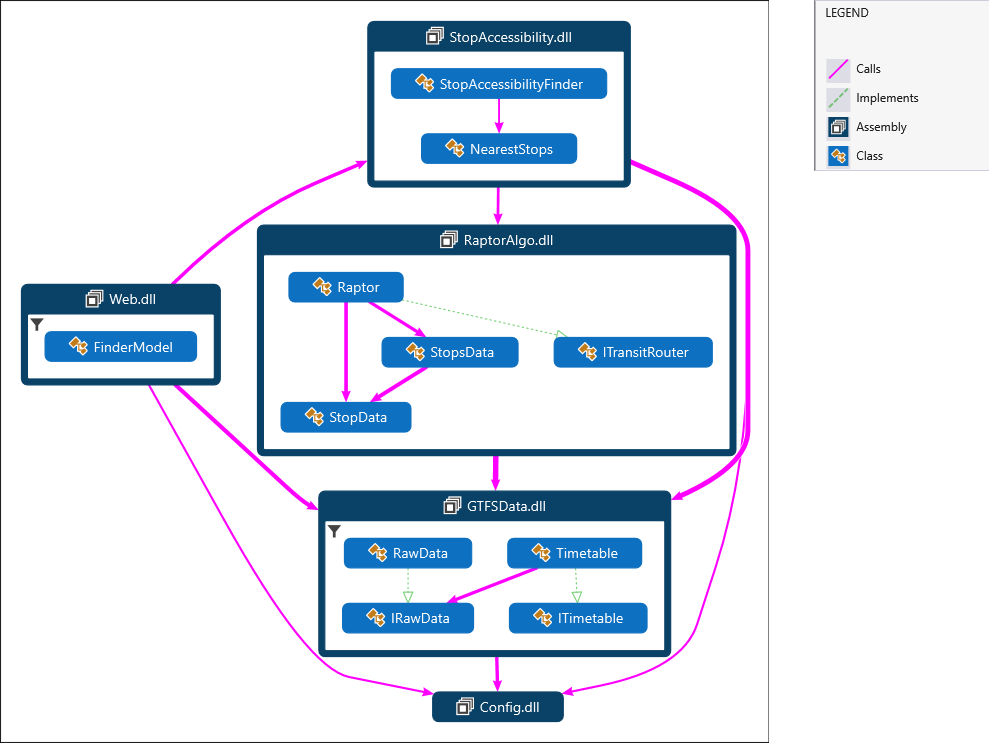
\includegraphics[width=\textwidth]{../img/codemap}
    \caption{Moduly aplikace a~jejich vzájemné propojení.}
    \label{fig:library-modules}
\end{figure}

Knihovní část projektu testujeme pomocí Unit Testů, psaných nástrojem XUnit. Testy pokrývají všechna základní použití knihovny, doplněné o~testy založené na chybách nalezených při vývoji.

% TODO: --------------v

% mozne rozsireni: o automaticky timezone
    % nepouziva Agency - alternativa v configu -- mozne rozsireni automatizaci


% update dat na webu---